%------------------------------------------------------------------------------
\chapter{The Standard Model and the top quark}
\label{sec:SM1}
%------------------------------------------------------------------------------
In this chapter, the fundamental framework of elementary particle physics and the basic concepts are introduced. Furthermore, a more detailed  description of the top-quark is given and the interests in the top-quark mass are motivated.  

\section{Particles, forces and fields}\label{key:SM 2}
% Standard model of physics
% Author: Carsten Burgard

%%%<


\begin{figure}
	\centering



\newcommand\particle[7][white]{%
	\begin{tikzpicture}[x=1cm, y=1cm]
	\path[fill=#1,] (0.1,0) -- (0.9,0)
	arc (90:0:1mm) -- (1.0,-0.9) arc (0:-90:1mm) -- (0.1,-1.0)
	arc (-90:-180:1mm) -- (0,-0.1) arc(180:90:1mm) -- cycle;
	\ifstrempty{#7}{}{\path[]
		(0.6,0) --(0.7,0) -- (1.0,-0.3) -- (1.0,-0.4);}
	\ifstrempty{#6}{}{\path[] (0.7,0) -- (0.9,0)
		arc (90:0:1mm) -- (1.0,-0.3);}
	\ifstrempty{#5}{}{\path[] (1.0,-0.7) -- (1.0,-0.9)
		arc (0:-90:1mm) -- (0.7,-1.0);}
	\draw[\ifstrempty{#2}{dashed}{black}] (0.1,0) -- (0.9,0)
	arc (90:0:1mm) -- (1.0,-0.9) arc (0:-90:1mm) -- (0.1,-1.0)
	arc (-90:-180:1mm) -- (0,-0.1) arc(180:90:1mm) -- cycle;
	\ifstrempty{#7}{}{\node at(0.825,-0.175) [rotate=-45,scale=0.2] {#7};}
	\ifstrempty{#6}{}{\node at(0.9,-0.1)  [nosep,scale=0.17] {#6};}
	\ifstrempty{#5}{}{\node at(0.9,-0.9)  [nosep,scale=0.2] {#5};}
	\ifstrempty{#4}{}{\node at(0.1,-0.1)  [nosep,anchor=west,scale=0.25]{#4};}
	\ifstrempty{#3}{}{\node at(0.1,-0.85) [nosep,anchor=west,scale=0.3] {#3};}
	\ifstrempty{#2}{}{\node at(0.1,-0.5)  [nosep,anchor=west,scale=1.5] {#2};}
	\end{tikzpicture}
}


	\begin{tikzpicture}[x=2cm, y=2cm]
	%\draw (-0.5,0.5) rectangle (4.4, -1.5);
	%\draw (-0.6,0.6) rectangle (5.0,-2.5);
	%\draw (-0.7,0.7) rectangle (5.6,-3.5);
	
	\node at(0, 0)   {\particle[blue!20!white]
		{$u$}        {up}       {$2.3$ MeV}{1/2}{$2/3$}{R/G/B}};
	\node at(0,-1)   {\particle[blue!20!white]
		{$d$}        {down}    {$4.8$ MeV}{1/2}{$-1/3$}{R/G/B}};
	\node at(0,-2)   {\particle[blue!20!white]
		{$e$}        {electron}       {$511$ keV}{1/2}{$-1$}{}};
	\node at(0,-3)   {\particle[blue!20!white]
		{$\nu_e$}    {$e$ neutrino}         {$<2$ eV}{1/2}{}{}};
	\node at(1, 0)   {\particle
		{$c$}        {charm}   {$1.28$ GeV}{1/2}{$2/3$}{R/G/B}};
	\node at(1,-1)   {\particle 
		{$s$}        {strange}  {$95$ MeV}{1/2}{$-1/3$}{R/G/B}};
	\node at(1,-2)   {\particle
		{$\mu$}      {muon}         {$105.7$ MeV}{1/2}{$-1$}{}};
	\node at(1,-3)   {\particle
		{$\nu_\mu$}  {$\mu$ neutrino}    {$<190$ keV}{1/2}{}{}};
	\node at(2, 0)   {\particle
		{$t$}        {top}    {$173.2$ GeV}{1/2}{$2/3$}{R/G/B}};
	\node at(2,-1)   {\particle
		{$b$}        {bottom}  {$4.7$ GeV}{1/2}{$-1/3$}{R/G/B}};
	\node at(2,-2)   {\particle
		{$\tau$}     {tau}          {$1.777$ GeV}{1/2}{$-1$}{}};
	\node at(2,-3)   {\particle
		{$\nu_\tau$} {$\tau$ neutrino}  {$<18.2$ MeV}{1/2}{}{}};
	\node at(3,-3)   {\particle[green!20!white]
		{$W^{\hspace{-.3ex}\scalebox{.5}{$\pm$}}$}
		{}              {$80.4$ GeV}{1}{$\pm1$}{}};
	\node at(4,-3)   {\particle[green!20!white]
		{$Z$}        {}                    {$91.2$ GeV}{1}{}{}};
	\node at(3.5,-2) {\particle[yellow!50!white!]
		{$\gamma$}   {photon}                        {}{1}{}{}};
	\node at(3.5,-1) {\particle[pink!50!white]
		{$g$}        {gluon}                    {}{1}{}{color}};
	\node at(5,0)    {\particle[gray!50!white]
		{$H$}        {Higgs}              {$125.1$ GeV}{0}{}{}};
%	\node at(6.1,-3) {\particle
%		{}           {graviton}                       {}{}{}{}};
	
	%\node at(4.25,-0.5) [force]      {strong force (color)};
	%\node at(4.85,-1.5) [force]    {electromagnetic force (charge)};
	%\node at(5.45,-2.4) [force] {weak nuclear force (weak isospin)};
	%\node at(6.75,-2.5) [force]        {gravitational force (mass)};
	
	\draw [<-] (2.5,0.3)   -- (2.7,0.3)          node [legend] {charge};
	\draw [<-] (2.5,0.15)  -- (2.7,0.15)         node [legend] {colors};
	\draw [<-] (2.05,0.25) -- (2.3,0) -- (2.7,0) node [legend]   {mass};
	\draw [<-] (2.5,-0.3)  -- (2.7,-0.3)         node [legend]   {spin};
	
	\draw [mbrace] (-0.8,0.5)  -- (-0.8,-1.5)
	node[leftlabel] {quarks};
	\draw [mbrace] (-0.8,-1.5) -- (-0.8,-3.5)
	node[leftlabel] { leptons};
	\draw [mbrace] (-0.5,-3.6) -- (2.5,-3.6)
	node[bottomlabel]
	{ fermions\\};
	\draw [mbrace] (2.5,-3.6) -- (4.5,-3.6)
	node[bottomlabel] {gauge bosons\\};
	
%	\draw [brace] (-0.5,.8) -- (0.5,.8) node[toplabel]         {stable };
	%\draw [brace] (0.5,.8)  -- (2.5,.8) node[toplabel]         {unstable };
	%\draw [brace] (2.5,.8)  -- (4.5,.8) node[toplabel]          {force carriers};
	\draw [brace] (4.5,.8)  -- (5.5,.8) node[toplabel]       {goldstone\\bosons };
	%\draw [brace] (5.5,.8)  -- (7,.8)   node[toplabel] {outside\\standard %model};
	
	\node at (0,.8)   [generation] {1\tiny st};
	\node at (1,.8)   [generation] {2\tiny nd};
	\node at (2,.8)   [generation] {3\tiny rd};
	\node at (2.8,.8) [generation] {\tiny generation};
	
	
	\end{tikzpicture}

	\caption{Graphical } \label{fig:SM}
\end{figure}


  
%%% Local Variables: 
%%% mode: latex
%%% TeX-master: "../mythesis"
%%% End: 

\clearpage


On the most elementary scale, all known fundamental matter can be described by the Standard Model of Particle Physics (SM)~\cite{Glashow:1961tr,Glashow:1970gm,Gross:1973ju,Politzer:1973fx,Politzer:1974fr,Salam:1964ry,Weinberg:1967tq}. This fundamental mathematical framework is a combined relativistic Quantum Field Theory (QFT), which describes the interaction of all known elementary particles by the fundamental forces, gravity excluded.
In this theory the particles are represented by fields $\Psi$ ($\bar{\Psi}$  corresponds to the antiparticle). The evolution of these fields is given by the Euler-Lagrange equations, which can be determined by Hamilton's principle of stationary action $\delta S[\mathscr{L}] \!= 0 $, where $S[\mathscr{L}] $ denotes the action functional, which depends on the Lagrangian density $\mathscr{L} $. Claiming the invariance of
$\mathscr{L}$ under local gauge transformations, leads to the introduction of a  vector boson set as force mediators.

 In summary, there are currently, as displayed in~\cref{fig:SM}, three generations of fermions (spin-1/2), distinguishable into quarks and leptons. Each generation consists of an up- and a down-type quark, a charged lepton and a corresponding light neutrino. While the charged leptons carry exactly one unit of elementary charge $e$, the quarks have  a irrational number of the electromagnetic charge. Furthermore, the quarks also carry the so-called colour charge, which is related to the strong interaction. The fermion generations are ordered by the increasing mass values.
In addition, there are thirteen bosonic particles in the SM, twelve vector bosons (spin-1) and one scalar goldstone boson (spin-0).
 The charged $W^{\pm}$-boson and the two uncharged vector bosons, the $Z^0$-boson and the photon $ \gamma$, are the participants in electroweak (EW) processes, while the strong force interacts via eight massless gluon fields $g$. The scalar Higgs boson is the latest discovered particle of the Standard Model and represents the mass generating mechanism of the particles in the SM framework. An overview of the most important properties of all SM particles is shown in~\cref{tab:T21}. 
 
 The  mass values of the quarks and the charged leptons are significant, compared to the neutrino masses, where only lower limits could be established so far.
 \begin{center}
\captionof{table}{ Summary of important properties of the SM particle content. The upper part displays the current mass value $m_i$  for the different fermion generations ($i = I, II, III$), the electromagnetic charge $Q$ in units of the elementary charge $e$ and the third component of the weak isospin $I_3$. The mass values for the gauge and goldstone bosons are shown below, together with the spin, the electromagnetic charge and the colour charge of the strong interaction. All values refer to 2017 and are taken from~\cite{Olive:2016xmw}. }\label{tab:T21}

	
\vspace{0.3cm}	
	

\begin{tabular}{>{\centering}m{1cm} >{\centering}m{2.6cm} >{\centering}m{0.5cm} >{\centering}m{2.3cm} >{\centering}m{0.8cm}  >{\centering}m{2.5cm} >{\centering}m{0.1cm} >{\centering}m{1cm}>{\centreing}m{0.7cm}} \toprule
%\emph{ }&		&	\emph{}&		\emph{fermions}&		\emph{} & & &\\  
%\midrule
				 		Fermions							&	m$_I$ / [MeV]                &          		          &	m$_{II}$ / [MeV]                       &	                                      &	m$_{III}$ / [MeV]                   &       &  Q / [e]    &    I$_3$  &                      
							 										\midrule
			\begin{center}				 	\begin{pmatrix} $u$ \\ $$d \end{pmatrix}  \end{center}    &    \begin{tabular}{1} \small 2.2^{+~0.6}_{-~0.4} & \small 4.7^{+~0.5}_{-~0.4}  \end{tabular} &   	\begin{pmatrix} $c$ \\ $s$ \end{pmatrix} &  \begin{tabular}{1}\small 1.27(0.03)\cdot~10^3 & \small 96^{+~8}_{-~4}   \end{tabular} & \begin{pmatrix} $t$ \\ $b$ \end{pmatrix}  &  \begin{tabular}{1} \small 173.1(0.6)\cdot~10^3  & \small 4.18^{+~0.04}_{-~0.03}~\cdot 10^3  \end{tabular} & &\begin{tabular}{1}+2/3 & -1/3 \end{tabular} & \begin{tabular}{1}+1/2 & -1/2 \end{tabular}   &
			\begin{center}				 	\begin{pmatrix} $e$ \\ $\nu_e$ \end{pmatrix}  \end{center}    &    \begin{tabular}{1} \small 0.5109989461(31) & \small<~2\cdot10^{-6} \end{tabular} &   	\begin{pmatrix} $\mu$ \\ $\nu_{\mu}$\end{pmatrix} &  \begin{tabular}{1}\small 105.6583745(24) &\small <~0.19\cdot10^{-6}~\end{tabular} & \begin{pmatrix} $\tau$ \\ $\nu_{\tau}$ \end{pmatrix}  &  \begin{tabular}{1} \small 1776.86(0.12) & \small <~18.2\cdot10^{-6} \end{tabular} & \begin{tabular}{1}  &  \end{tabular} & \begin{tabular}{1}-1 & 0 \end{tabular}  & \begin{tabular}{1} -1/2 &+1/2 \end{tabular}  &
%							 &  	\begin{pmatrix} e \\ $\nu_e$ \end{pmatrix}    &    \begin{tabular}{1} masse & mass \end{tabular} &   	\begin{pmatrix} u \\ d \end{pmatrix} &  \begin{tabular}{1} masse & mass \end{tabular} & \begin{pmatrix} u \\ d \end{pmatrix}  &  \begin{tabular}{1} masse & mass \end{tabular} & \begin{tabular}{1} masse & mass \end{tabular} & \begin{tabular}{1} masse & mass \end{tabular}  &\\
\midrule
 Bosons & & &m / [MeV]&  &Spin& & Q / [e]&Colour&
\midrule
W^{\pm} & & & 80.385(0.015)\cdot 10^3& &1 & & $\pm$1&no&
Z^0 & & & 91.1876(0.0021)\cdot 10^3 & & 1& & 0& no&
$\gamma $ &  & &< 1\cdot 10^{-24}& &1 & & 0 & no&
$g$ &  & & 0& & 1& &0 & yes&
$H^0$ &  & & 125.09(0.24)\cdot 10^3& &0& & 0 &no &








\bottomrule
\end{tabular}

\end{center}

\vspace{0.1cm}




 


 
\section{Fundamental forces and symmetry breaking}
In terms of a field theory, the SM basically combines Quantum Chromo Dynamics (QCD), the theory of the strong interaction, and the unified electroweak theory (EW). Both theories can be identified with a symmetry group.
The fundamental concept of the  elementary interactions rests on the idea, that the interactions can be mathematically expressed by  local gauge transformations:
\begin{equation}\label{trafo}
\Psi \longrightarrow \Psi'(x) =  e^{i\alpha(x)}\Psi(x).
\end{equation}  
This is the most general from of a finite local transformation with a phase factor $\alpha(x)$, whose specific functional form depends  on the chosen symmetry group. 
The cornerstone of the SM concept is that the corresponding Lagrangian densities are invariant under the local gauge transformations.  
In order to achieve this invariance, covariant derivatives  and the above mentioned vector gauge fields are introduced. Nevertheless, the fact that the gauge bosons are massive, violates the locale gauge invariance. This contradiction can be solved by the concept of spontaneous symmetry breaking, bringing up the famous Higgs boson.

 Coming up next is a short introduction of QCD and the electroweak theory before a brief approach is taken to clarify the concept of symmetry breaking. This short introduction is based on the work of W. Hollik~\cite{Hollik:2010id}. 

\subsection{Quantum Chromo Dynamics}\label{QCD}
The interaction of massive spin-1/2 quarks and massless spin-1 gluons is described by the non-abelian gauge group $SU(3)_C$, where $C$  refers to the charge of the strong interaction, called colour. The corresponding Lagrangian density is given by
\begin{equation}\label{LQCD}
\mathscr{L}_{QCD} = - \frac{1}{4} F^a_{\mu\nu}F^{\mu\nu}_a +\sum_{f}\bar{\Psi}_f^C(i\gamma^{ \mu}D_{\mu}-m_f)\Psi_f^C, \hspace{0.5cm}\text{with}
\end{equation}
\begin{equation}\label{Fieldtensor}
F^a_{\mu\nu} = \partial_{\nu}G_{\mu}^a - \partial_{\mu}G_{\nu}^a+g_sf^{abc}G_{\mu}^bG_{\nu}^c.
\end{equation}
In the first term $F^a_{\mu\nu}$  is the field strength tensor, derived from eight massless gluon fields $G_{\mu}^a$. $\partial_{\nu}$ denotes the derivative of the four-vectors\footnote{$\partial_{\nu}$ =($\partial_{t}$, $\partial_{1}$, $\partial_{2}$, $\partial_{3}$).}. The interaction strength is determined by the strong coupling constant $g_s$.  $f^{abc}$ are the structure constants of the strong interaction, with the indices $a,b,c$ running over all eight degrees of freedom of the $SU(3)_C$ group. The number of degrees of freedom results from the eight generators $T^a$ of the $SU(3)_C$  group in its fundamental representation, which can be expressed by the Gell-Mann matrices $T^a=\lambda^a/2$, with the Lie-algebra:
 \begin{equation}
[T^a,T^b]=if^{abc}T^c.
\end{equation}
 The last term of the Lagrangian sums over all quark flavours ($f= u,d,...$), with the quark fields $\Psi_f^C$ and masses $m_\text{f}$\footnote{These mass terms break the weak isospin and hypercharge symmetry. The mass generation mechanism to solve these problems will be introduced in \cref{Higgsm}. }. The quarks are grouped to $SU(3)_C$ colour triplets ($C$ = red, green, blue), while the corresponding antiquarks belong to the conjugated fundamental $SU(3)_C$ representation and carrying matching anticolours. In contradiction to the photon, the force carrier of the electromagnetic force, the gluons themselves are carrying the colour charge, which results in gluon-gluon self-coupling. 
In order to keep the  QCD-Lagrangian invariant under local $SU(3)_C$ gauge transformations, the covariant derivative 
\begin{equation}\label{Kovariant}
D_{\mu}=\partial_{\mu}+ig_sT^aG_{\mu}^a,
\end{equation} 
is introduced.

\noindent The QCD-coupling strength can be further characterized by  $\alpha_s = g_s^2/4\pi$, which depends  on the energy scale and therefore can not be treated as constant. Furthermore, to compensate ultraviolet divergences, a renormalization with a specific reference scale $\mu(Q^2)$ has to be made. A convenient choice is the renormalization to the $Z^0$-boson mass with a measured coupling of $\alpha_s(Q^2=M_Z^2) = 0.1184 \pm 0.0031$~\cite{Bethke:2000ai}. In addition, for short distances (= high energies) the strength of the strong coupling becomes sufficiently small and one observes free particle like behaviour, which is known as asymptotic freedom. On the other hand, in the low energy regime (= long distances), the coupling is differently and can be expressed by 
\begin{equation}\label{alphas}
\alpha_s(Q^2)=\frac{12\pi}{(33-2N_f)~\text{ln}(\frac{Q^2}{\Lambda_{QCD}^2})},
\end{equation}
where $N_f$ refers to the number of participating quark flavours at the energy $Q^2$. $\Lambda_{QCD}$ is of the order $O(200~\text{MeV})$ and represents the energy scale where the perturbation theory  breaks down, due to the ultraviolet divergences. As ~\cref{alphas} suggests, the coupling strength increases with decreasing energy, resulting in the confinement of the quarks. Consequently, quarks and gluons do not propagate over macroscopic distances and can therefore only be observed via the hadrons -the colour neutral quark bound states- which are experimentally accessible. One general refers this as confinement, where the hadrons represent the singlet states of  the $SU(3)_C$-group and are either baryons, consisting of three quarks or antiquarks,  or mesons which are quark-antiquark pairs. 
























\subsection{The electroweak force}\label{EW}
The electromagnetic force, described by Quantum Electrodynamics (QED), and the weak interaction are unified by the theory of Glashow, Weinberg and Salam (GSW)~\cite{Glashow:1961tr,Weinberg:1967tq,Salam:1964ry}, which is based on the $SU(2)_L\times U(1)_Y$ symmetry group product. The invariance requirement of the corresponding Lagrangian density leads to the introduction of the four well known physical vector gauge bosons $W^{\pm}, Z^0$ and $\gamma$.

In the framework of the weak interaction with its fundamental representation expressed by the $SU(2)$ group, the fermions are grouped in left-handed doublets and right-handed singlets of the weak isospin $I_3$
\footnote{The term handedness refers to the fact that the fields can be split into a right-handed and left-handed part, which are defined by the eigenvalues of the projection operator $P_{L/R}= \frac{(1\pm \gamma^5)}{2}$ with the Dirac matrix $\gamma^5$.}. 
A striking observation is the maximal violation of the parity conservation by weak interactions.\footnote{The sign changing transformation of space coordinate $\vec{r}$ is called parity. }
Consequently only left-handed fermions and right-handed antifermions contribute in weak interaction processes.  Furthermore, the  quark mass eigenstates ($d,s,b$), which couple to the gauge fields, are not identical with the weak isospin eigenstates of the quarks ($d',s',b'$). These different states are connected by the  Cabbibo-Kabayashi-Maskawa (CKM) matrix \cite{Cabibbo:1963yz, Kobayashi:1973fv}:
\begin{equation}\label{CKM}
\begin{pmatrix}
d'\\
s'\\
b'
\end{pmatrix}
=
 \begin{pmatrix}
\rm  V_{ud} &\rm V_{us} &\rm V_{ub}\\
\rm  V_{cd} &\rm V_{cs} &\rm V_{cb}\\
\rm  V_{td} &\rm V_{ts} &\rm V_{tb}
\end{pmatrix} 
\cdot
\begin{pmatrix}
d\\
s\\
b
\end{pmatrix}.
\end{equation}
The CKM matrix elements can only be determined by experimental measurements~\cite{Olive:2016xmw}. The diagonal elements are measured close to unity.  Following from the quark flavour mixing in the weak interaction, one can observe quark flavour oscillations and the violation of the CP\footnote{CP represents the product of charge conjugation and parity.} conservation.

Compared to the weak interaction, QED does not distinguish between the left and right handed particles. In the GSW model, electromagnetic interactions are taken into account by the $U(1)$ symmetry group, where the weak hypercharge $Y$ is added as an additional quantum number connected to the electromagnetic charge $Q$ and the weak isospin $I_3$ via the Gell-Mann–Nishijima formula:
\begin{equation}
Q = I_3 + \frac{Y}{2}.
\end{equation}

 The unified electroweak theory is described by  $SU(2)_L\times U(1)_Y$  and has the four group generators $I_a$ with $a$ = 1,2,3 and $Y$, with the Lie-algebra:
\begin{equation}
[I_a,I_b]=i\epsilon_{abc}I_c  \hspace{1.0cm} \text{and} \hspace{1.0cm} [I_a,Y]= 0.
\end{equation}
$\epsilon^{abc}$ denotes the Levi-Civita symbol with the indices running over the triplet ($a,b,c = 1,2,3$).
 The corresponding  Lagrangian for the unified electroweak interaction theory takes the following functional from:
\begin{equation}\label{LGSW}
 \mathscr{L}_{GSW} = -\frac{1}{4} F^a_{\mu\nu}F^{\mu\nu}_a -\frac{1}{4} f_{\mu\nu}f^{\mu\nu}  +\sum_{f}\bar{\Psi}_{f_R}(i\gamma^{ \mu}D_{\mu_R})\Psi_{f_R}  +\sum_{f}\bar{\chi}_{f_L}(i\gamma^{ \mu}D_{\mu_L})\chi_{f_L}.
\end{equation}

 In order to keep the Lagrangian gauge invariant, four gauge vector fields are introduced, a boson triplet $\vec{W} = (W_1,W_2,W_3)^T$ and a boson singlet $B_0$. The field strength tensors of the GSW-Model, which describe the kinematics of the fields, are:   

 \begin{equation}\label{FieldtensorW}
 F^a_{\mu\nu} = \partial_{\nu}W_{\mu}^a - \partial_{\mu}W_{\nu}^a+g\epsilon^{abc}W_{\mu}^bW_{\nu}^c,
 \end{equation}
 \begin{equation}\label{FieldtensorB}
 f_{\mu\nu} = \partial_{\nu}B_{\mu}- \partial_{\mu}B_{\nu}.
 \end{equation}

 Fermion interactions are taken into account with the last terms of the  $\mathscr{L}_{GSW} $. The fileds $\Psi_{f_R}$ describe the interaction of the right-handed fermion singlets, while the ${\chi}_{f_L}$ fields take care of the left-handed fermion doublets. Furthermore, two different covariant derivatives are introduced with respect to the orientations of the fermions. Left-handed charged fermions take part in weak- and electromagnetic processes, which leads to:    
\begin{equation}\label{Kovariant2}
D_{\mu_L}=\partial_{\mu}+ig'\frac{Y_L}{2}B_{\mu} + ig\vec{I}\cdot \vec{W_{\mu}}.
\end{equation}
All four gauge fields  keep the required invariance under the corresponding gauge transformations. The coupling strength of the interactions is given by the constants $g$ and $g'$. In contrast to the left-handed fermions, the covariant derivative takes a much simpler from for right-handed fermions:
\begin{equation}\label{Kovariant1}
D_{\mu_R}=\partial_{\mu}+g'\frac{Y_R}{2}B_{\mu}.
\end{equation} 

The four vector fields, appearing in gauge theory, can easily be related to the physical quantities which have been studied extensively. 
The observed $W$-bosons, mediating the charged current (CC), are given by the combination
\begin{equation}\label{EWtrafo1}
 W^{\pm}_\mu = \frac{1}{2}(W^{1}_\mu\pm iW^{2}_\mu),
\end{equation}
of the two gauge fields $W^{1}_\mu$ and $W^{2}_\mu$. The $Z^0$-boson and $\gamma$ (represented in QED as $A_\mu$) are mediating the neutral current (NC) and can be constructed from the two gauge fields $B_{\mu}$ and $W_{\mu}^{0}$ by an orthogonal rotation:
\begin{equation}\label{EWtrafo2}
\begin{pmatrix}
A_\mu\\
Z^0_\mu
\end{pmatrix}
=
\begin{pmatrix}
\text{cos}\Theta_W & \text{sin}\Theta_ W \\
-\text{sin}\Theta_W & \text{cos}\Theta_W  \\

\end{pmatrix}
\cdot 
\begin{pmatrix}
B_\mu\\
W^0_\mu
\end{pmatrix},
\end{equation}
 $\Theta_W$ is the Weinberg angle, which relates the two coupling constants $g$ and $g'$ with the weak hypercharge $Y_L$:
\begin{equation}\label{Weinber2}
\text{cos} \Theta_W = \frac{g}{\sqrt{g^2+g'Y^2_L}}.
\end{equation} 

The experimentally observed neutral vector bosons can be expressed in terms of the gauge fields and the coupling constants: 

\begin{equation}
A_\mu = \frac{gB_\mu -g'Y_LW_\mu^0}{\sqrt{g^2+g'Y^2_L}} ~~~~\mathrm{and} ~~~~Z_\mu^0 = \frac{gW_\mu^0 +g'Y_LB_\mu}{\sqrt{g^2+g'Y^2_L}}.
\end{equation}

The GSW-Model shows in a very elegant way the unification of two interactions, by introducing just a minimal set of gauge fields. Nevertheless, this theory is not able to deal with massive gauge bosons, because mass terms inside the Lagrangian would break its gauge symmetry. However, since measurements have shown that the $W^\pm$ and the $Z^0$-boson are in fact very massive objects, the implementation of a mass generation mechanism has been a cornerstone of research in elementary particle physics over the past decades.

 In following sections of this thesis, the gauge fields ($W^\pm$, $Z^0$) are just denoted by $W$ and $Z$.



 
\subsection{The Higgs mechanism}\label{Higgsm}
\begin{figure}[h]
	\centering
	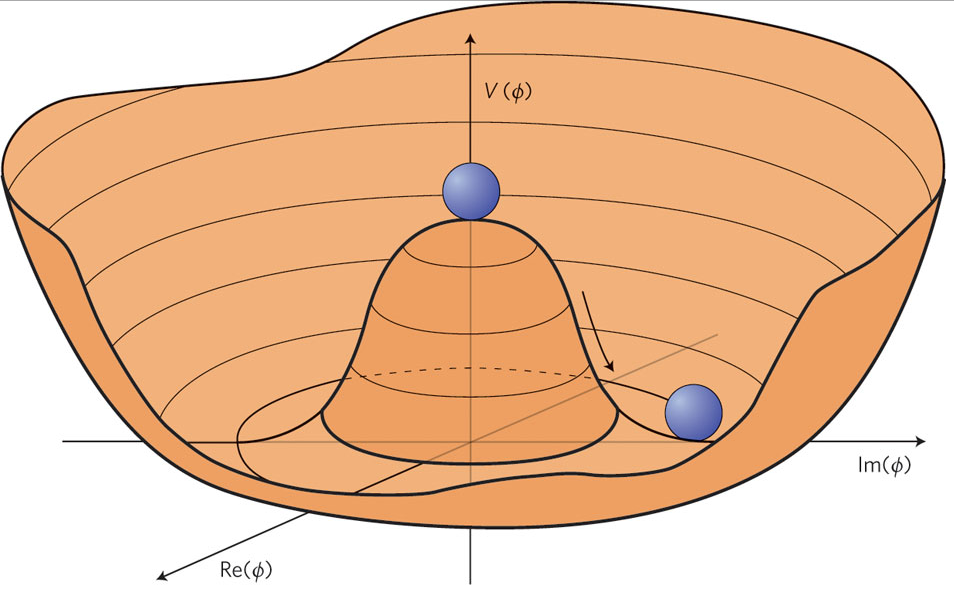
\includegraphics[width=0.4\linewidth]{Pics/cp1/Higgs}
	\caption{Illustration of the Higgs potential for $\mu^2>0 $ and $\lambda>0$ from ~\cite{Ellis:2013jnq}. The complete set of vacuum states is given by the circular potential minimum. Excitations in the transversal direction lead to the introduction of a massive spin-0 particle, the Higgs boson.}
	
	\label{fig:Higgs}
\end{figure}

The non-vanishing masses of the electroweak gauge bosons, one of the biggest issues inside the SM framework, has been solved by Brout, Englert, Guralnik, Hagen, Kibble and Higgs~\cite{Higgs:1964ia,Higgs:1964pj,Guralnik:1964eu,Englert:1964et}, by the introduction of an additional complex scalar field - the so-called Higgs field- as a weak isospin $I_3$ doublet
\begin{equation}
\Phi(x) =
 \begin{pmatrix}
	\phi^{\dagger}(x)\\
	\phi_0(x)
\end{pmatrix},
\end{equation} 
  with the hypercharge $Y$=1. The coupling of $\Phi$ to the electroweak gauge fields is realized by adding
  \begin{equation}\label{Lhiggs}
  \mathscr{L}_{Higgs} = (D_{\mu}\Phi )^{\dagger}(D^{\mu}\Phi)-V(\Phi,\Phi^{\dagger})
  \end{equation}
  to the total Lagrangian of the Standard Model.
  The covariant derivatives $D_{\mu}$ are introduced in~\cref{Kovariant2} and include the coupling to the electroweak gauge fields $\vec{W}_{\mu}$ and $B_{\mu}$.
  In addition the potential  
  \begin{equation}\label{HiggsV}
  V(\Phi,\Phi^{\dagger}) = -\mu^2\Phi^{\dagger}\Phi + \frac{\lambda}{4}(\Phi^{\dagger}\Phi)^2, 
  \end{equation}
  with the two real constants $\mu^2$ and $\lambda$ is added.  This so-called Higgs potential
  is symmetric under rotations around the z-axis and contains the self interaction of the Higgs field. Its characteristic shape (see~\cref{fig:Higgs}) is determined by choosing $\mu^2>0 $ and $\lambda>0$. In the vacuum ground state, the potential has a minimum at a non-zero value $\Phi\neq$0. Furthermore,  $V(\Phi,\Phi^{\dagger})$ takes its minimum value in the complex plane w.l.o.g. for all field configurations satisfying~$\Phi^{\dagger}\Phi=2\mu^2/\lambda$. By constraining the field configuration to be real and free of electrical charge, one gets for  the vacuum expectation value:
\begin{equation}
\langle\Phi_0\rangle = \frac{1}{\sqrt{2}}
\begin{pmatrix}
0\\
\nu
\end{pmatrix}
, \text{ \hspace{0.5cm} with}~ \nu = \frac{2\mu}{\sqrt{\lambda}}.
\end{equation}


 In general $\mathscr{L}_{Higgs}$ has the $SU(2)_L\times U(1)_Y$ symmetry of the electroweak gauge theory. However, this is not the case for the groundstate $\langle\Phi\rangle _0$ of the system, which contains only the gauge symmetry of the electromagnetic force $U(1)_Y$. Thus the  actual symmetry of the Lagrangian is  broken, which is known as \textbf{spontaneous symmetry breaking}.


Deviations of the Higgs potential from its groundstate,  like $\phi_0(x)=\nu + H(x)+ i\chi(x)$, allow to express the potential in the following from:
\begin{equation}
  V(\Phi,\Phi^{\dagger})=\mu^2H^2+\frac{\mu^2}{\nu}H^3 + \frac{\mu^2}{4\nu^2}H^4.
\end{equation}
The contributions from $\chi(x)$ and $\phi^{\dagger}$ are massless unphysical degrees of freedom and can be eliminated by choosing an appropriate gauge transformation. $H$ leads to the introduction of a scalar particle (the Higgs boson) with a mass of
$m_{\text{H}}=\sqrt{2}\mu$
and self coupling vertices of the Higgs field.

The coupling of the gauge fields $\vec{W}_{\mu}$ and $B_{\mu}$ and the Higgs field arises from the  kinetic term of the Lagrangian~\cref{Lhiggs}. With the transformations~\cref{EWtrafo1,EWtrafo2}, the masses of the observed bosons are:
\begin{equation}
 m_W=\frac{1}{2}g\nu ~~~~ \mathrm{and} ~~~~m_Z=\frac{1}{2}\sqrt{g^2+g'^2}\nu. 
\end{equation}  
 
 
 The Higgs mechanism is also able to explain the observation of massive charged fermions by Yukawa coupling between the Higgs field and the charged fermion fields.
This can be expressed with the additional term:  
\begin{equation}
\mathscr{L}_{Yukawa}=\sum_{f}m_f(\bar{\Psi}_f\Psi_f-\bar{\Psi}_f\Psi_f H).
\end{equation} 

In this formula, the sum runs over the massive fermions, represented by the fields $\Psi_f$ and $\bar{\Psi}_f$. The fermion mass terms are related to the Yukawa coupling via individual coupling constants $G_f$, which are proportional to the fermion masses: 
\begin{equation}\label{Higpro}
G_f = \frac{\sqrt{2}}{\nu} m_f.
\end{equation} 

The Standard Model is not able to predict the mass of the Higgs boson $m_H$, as well as the different Yukawa coupling constants (or the fermion masses), which therefore have to be determined by measurements. The discovery of the Higgs boson in the year 2012 by the ATLAS and CMS collaborations~\cite{Aad:2012tfa,Chatrchyan:2012xdj}, was the fist evidence  for the Higgs mechanism and has been a milestone for the Standard Model. Currently the Higgs boson and its properties are the subject of intense studies at the LHC experiments. 
























\section{Relevance of the top quark}\label{Relevanz}

The first experimental evidence of top quarks from the CDF~\cite{Abe:1995hr} and the $D \emptyset$~\cite{Abachi:1995iq} collaborations in 1995, was a tremendous success in the field of particle physics. 
The production of top-quarks was observed in proton-antiproton collisions at a center-of-mass energy of 1.8~TeV. The existence of top quarks was already predicted 1977, as the weak isospin partner of the bottom quark~\cite{Herb:1977ek}. 

The top quark contributes noticeably to higher-order (HO) corrections e.g. in perturbation scattering theory.  From an experimental point of view, these HO corrections offer the possibility to perform observations at energy scales even higher than the center-of-mass energy of the actual experiment. Therefore, indirect particle searches can be performed by testing particle properties without directly observing them. This unique feature was used, together with precision measurements at the $e^+e^-$-collider LEP\footnote{Large Electron-Positron Collider.}, to constrain the top-quark mass to a range of 173$^{+18}_{-20}$~GeV.~\cite{LEPEW:1994aa}
\begin{figure}[h]
	\centering
	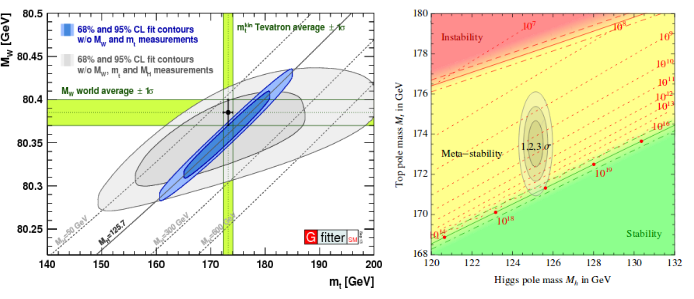
\includegraphics[width=0.9\linewidth]{Pics/Relevanz}
	\caption{Left: electroweak fit of the SM from ~\cite{Baak:2012kk}. $m_{\text{W}}$ is displayed vs $m_{\text{top}}$ with the direct measurements marked green. The  counters show the fit results for the indirect measurements of both masses, with the measured $m_{\text{H}}$ excluded (grey) and fixed (blue).
		Right: phase diagram of the EW vacuum in the $m_{\text{H}}-m_{\text{top}}$ plane from~\cite{Buttazzo:2013uya}. The plane is divided into regions of absolute stability, meta-stability and instability. The grey contour represents the area under experimental investigation.}
	\label{fig:Relevanz}
\end{figure}

With the discovery of the Higgs boson and the measurement of its mass $m_{\text{H}}$, all fundamental parameters of the SM are known and have been used for testing the self-consistency of the SM by global electroweak fits, as displayed in \cref*{fig:Relevanz} (left). The contours (gray/blue) belong to the 68\% and 95\% confidence level (CL) and result from scans  over fits of the $W$-boson mass $m_{\text{W}}$ vs the top-quark mass $m_{\text{top}}$ with a fixed $m_{\text{W}}$. The green bands mark the results from direct measurements of $m_{\text{W}}$ and $m_{\text{top}}$. 
Additionally, the dashed lines represent values for the Higgs mass ($m_{\text{H}}$) obtained from SM constrains, while the grey contours display the results of the indirect $m_{\text{W}}$ and $m_{\text{top}}$ determination, which agrees, within all uncertainties, quite well with the direct results for $m_{\text{W}}$ and $m_{\text{top}}$.
Despite the inclusion of the measured  Higgs mass (solid line), which leads to a significant reduction of the obtained contour (blue contour), the results still confirm the direct observations. This is a good  example for the remarkable consistency of the SM and the important role of $m_{\text{top}}$ inside this framework.~\cite{Baak:2012kk}



Furthermore, with its unusually high mass close to the electroweak symmetry breaking scale, the top quark plays a special role in several theoretical models, e.g. in top-colour models~\cite{Hill:1991at,Hill:1994hp}, where the  gauge extension of the SM is considered in the context of dynamical electroweak symmetry breaking~\cite{Bardeen:1989ds}. 

Moreover, the top-quark mass itself might be sensitive to new physics beyond the SM (BSM). There are several BSM theories, predicting the decay of heavy unstable exotic particles into top quarks that might result into contributions, which can be observed in higher-order corrections (see for example \cite{Kong:2014jwa}).


Finally, the top-quark mass, together with the Higgs boson mass, determines the different phases of the electroweak vacuum in the SM. In~\cref{fig:Relevanz} (right), the stable, metastable and instable regions of the EW vacuum are displayed.  The most interesting experimental region of the top-quark and the Higgs boson mass is marked by the grey contours for different CL levels. The dashed lines denote the uncertainties of the strong gauge coupling and the theoretical errors, while the dotted contour line displays the instability scale $\Lambda$.
The grey contours mark the region under current experimental investigation, where the vacuum state lies in a critical region between the stable and the metastable state. More precise measurements are needed, in order to further investigate this region.~\cite{Buttazzo:2013uya}



As already mentioned, the mass value of the top quark is  a fundamental parameter of the SM and therefore particularly interesting in terms of physic analyses. For this measurement, one is interested to determine $m_{\text{top}}$ from top-quark pairs. In general, there are basically two main experimental methods, which are used to determine the top-quark mass directly from the $t\bar{t}$ final state:


\begin{itemize}
	
	\item The first method is the so-called \textbf{matrix element method}, where the top-quark mass is determined by a maximum likelihood approach. An event by event probability is calculated, depending on the assumed results of the measurements, i.e. of $m_{\text{top}}$, using the leading-order matrix element. The evaluated probability defines the chances to have an $t\bar{t}$ event, with the assumed $m_{\text{top}}$ value. From these probability density functions, the likelihood and finally top-quark mass are computed.~\cite{Castro:2014cva}   
	
	\item The analysis presented here, is based on the \textbf{template method}. Monte Carlo based distributions of kinematic variables are simulated for different mass values $m_{	\text{top}}^{MC}$. These distributions are fitted to analytical functions and parametrized as probability density functions,  depending on the mass value. This allows the computation of a likelihood value and the extraction of the $m_{\text{top}}^{MC}$ value in an unbinned maximum likelihood fit.   
\end{itemize}

 Both analysis methods use the  mass concept corresponding to the MC simulated distributions. The main difficulty is the relation to  theory, since  the $m_{	\text{top}}^{MC}$ definition does not take the  renormalization into account, while this plays an  important role in the different theoretical approaches. 











   

\section{Top-quark production}
In the Standard Model, top quarks can be produced either as single particles 
(single tops) via electroweak processes or as a quark pair from strong interactions, which lead to a pair of a top and an antitop quark ($t\bar{t}$).    

\subsection{Single top-quark production}
The production of single top quarks was first observed at the Tevatron 2009~\cite{Abazov:2009ii,Aaltonen:2009jj}. There are three possible single top production channels. Their Feynman diagrams in leading-order (LO) are displayed in~\cref{fig:single}.


\begin{figure}[h]
	\centering
	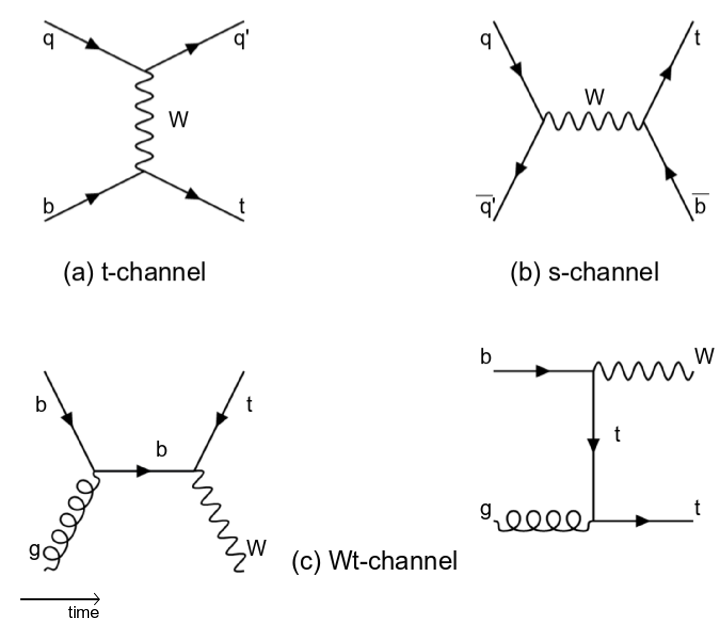
\includegraphics[width=0.5\linewidth]{Pics/cp1/single}
	\caption{Leading-order single top production in the three different channels s, t and Wt.} 
	\label{fig:single}
\end{figure}

 The \textbf{t-channel} process~\cref{fig:single} (a) is characterized by the transition of a bottom quark $b$ into a top quark, while a virtual $W$-boson is exchanged with a lighter quark or antiquark. This channel is the most significant contributor to the overall production.

The smallest production of single top quarks at the LHC arises from the \textbf{s-channel}~\cref{fig:single} (b). A quark and antiquark produce a virtual $W$-boson, decaying into a top and an antibottom quark (respectively into an antitop and a bottom quark).

Moreover, at the LHC, single top quarks can also be produced in the \textbf{Wt-channel}. In this channel, a $W$-boson is radiated from a bottom (anti-bottom) quark.

The  predicted production cross-sections of single-top quarks are calculated  for proton-proton collisions at a centre-of-mass energy of $\sqrt{s}=13$~TeV, for a top quark mass of 172.5~GeV, with modern theory predictions with the Hathor v2.1 program~\cite{Aliev:2010zk,Kant:2014oha}. For the evaluation of the PDF and $\alpha_{s}$ uncertainties, the following PDF sets are added in quadrature: PDF4LHC~\cite{Botje:2011sn} with the MSTW2008 68\% CL NLO~\cite{Martin:2009bu,Martin:2009iq}, CT10 NLO~\cite{Lai:2010vv} and NNPDF2.3~\cite{Ball:2012cx}. The results, with the total uncertainties, are displayed in~\cref{tab:T23}.



\begin{center}
	\captionof{table}{Combined production cross-section of single quarks + antiquarks, taken from~\cite{single}.}\label{tab:T23}
	
	
	\vspace{0.3cm}	
	
	
\begin{tabular}{>{}m{4.0cm}>{}m{4.0cm}} \toprule
		
		Process& Cross-Section/[pb] \\
		
		\midrule
		t-channel	&216.99$^{+9.04}_{-7.71}$\\
		s-channel	&10.32$^{+0.40}_{-0.36}$\\
		Wt-channel	&71.7$^{+1.80}_{-1.80}$\\
		
		\bottomrule
	\end{tabular}
	
\end{center}


\noindent At the LHC, the cross-section for single top quarks differs from the cross-section for anti-top quarks. The asymmetry of the production cross-section for $t$  and $\bar{t}$ is related to the nature of proton-proton collisions, where the only source for antiquarks is the sea quark distribution of the proton. This reduces the chance of having an antiquark in the initial state dramatically. A good example is given by the results of the cross-section measurement in the t-channel at $\sqrt{(s)}$=13~TeV~\cite{Aaboud:2016ymp}: 
\begin{equation*}
\sigma_ {t_{ch}}(tq)= 156\pm 5~(\text{stat.})\pm 27~(\text{syst.}) \pm 3~(\text{lumi}.)~\text{pb}, 
\end{equation*}
\begin{equation*}
\sigma_ {t_{ch}}(\bar{t}q)= 91\pm 4~(\text{stat.})\pm 15~(\text{syst.}) \pm 2~(\text{lumi}.)~\text{pb}.
\end{equation*}

 

.   


\subsection{Top-quark pair production}
\begin{figure}[h]
	\centering
	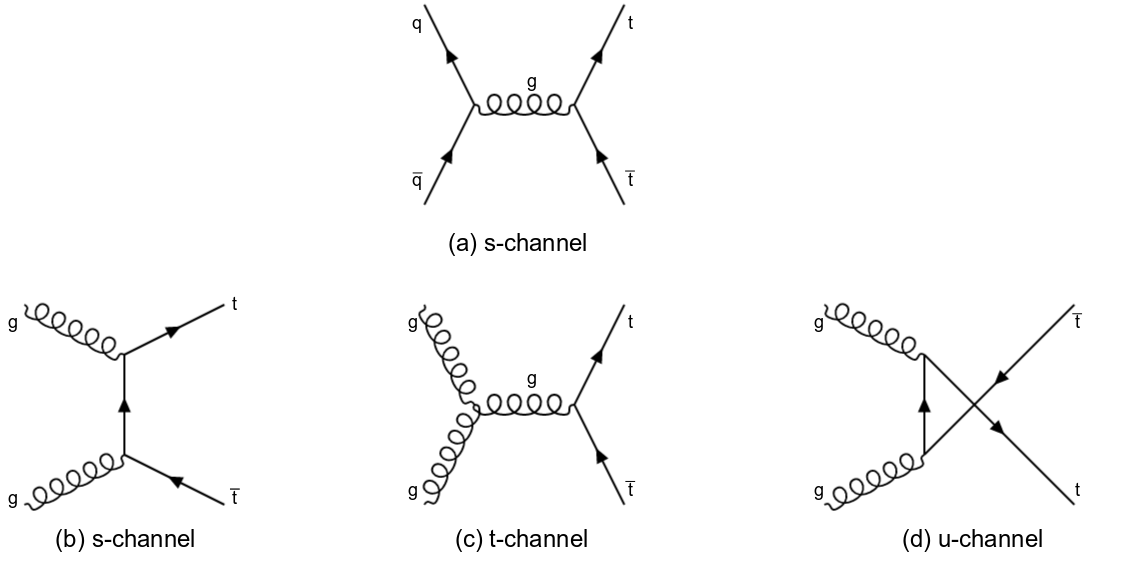
\includegraphics[width=0.70\linewidth]{Pics/cp1/ttbar}
	\caption{Leading-order top-quark pair production. Fig. (a) shows the quark- antiquark annihilation, fig. (b)-(d)  the gluon-gluon fusion.} 
	\label{fig:ttbar}
\end{figure}




\noindent The $t\bar{t}$-production processes can be distinguished into gluon-gluon fusion ($gg\rightarrow t\bar{t}$) and quark-antiquark annihilation ($q\bar{q}\rightarrow t\bar{t}$), which are both displayed in~\cref{fig:ttbar} in LO. At the LHC, the $t\bar{t}$-production is dominated by the gluon-gluon fusion ($\approx$ 90~\%). 
This issue has two reasons. One reason can be seen by considering the corresponding momentum fractions $x$ necessary to produce a top-quark pair at the LHC, which can be estimated under the assumption $x_i \approx x_j$:
\begin{equation}
x \geq 2m_{	\text{top}}/\sqrt{s}.
\end{equation}
With a center-of-mass energy of 13~TeV and an approximated top-quark mass of 173~GeV, this leads to $x \approx 0.027$. This low $x$ regime is, as shown by~\cref{fig:PDF}, highly dominated by the gluon PDF, which explains the strong gluon fusion contributions of the  $t\bar{t}$-production at LHC. 
 Furthermore, the only source for antiquarks are the sea distributions of the protons, while quarks are also present in the valence distributions. Therefore, the chances of interactions with antiquarks are slightly reduced. 
 
 
\noindent With modern theory predictions~\cite{Cacciari:2011hy,Beneke:2011mq,Baernreuther:2012ws,Czakon:2012zr,Czakon:2013goa} the $t\bar{t}$ production cross-section can be calculated with the Top++2.0 program~\cite{Czakon:2011xx}. For these calculations, the top-quark mass is assumed to be 172.5 GeV. 
 The predictions are computed with the corresponding scale (first term), PDF and $\alpha_s$ uncertainties (second term). For the latter one,  PDF4LHC~\cite{Botje:2011sn} with  MSTW2008 68\% CL NLO~\cite{Martin:2009bu,Martin:2009iq} are used,  as well as the CT10 NNLO~\cite{Gao:2013xoa} and NNPDF2.3~\cite{Ball:2012cx} PDFs. Furthermore, there is a mass uncertainty included (third term). For a center-of-mass energy of  13~TeV, top-quark pair production cross-section  is obtained to be (see~\cite{double}):
 

\begin{equation*}\sigma_ {t\bar{t}} = 831.76^{ +19.77 \hspace{7} +35.06 \hspace{7} +23.18}_{-29.20 \hspace{7} -35.06 \hspace{7} -22.45}~\text{pb}.
\end{equation*}



 




\begin{figure}[h]
	\centering
	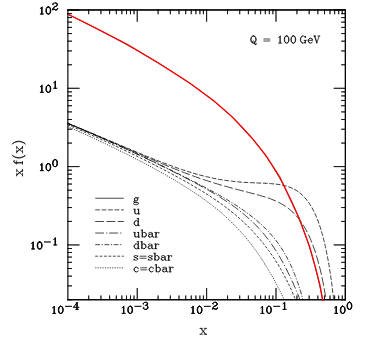
\includegraphics[width=0.55\linewidth]{Pics/cp1/PDF.png}
	\caption{ CTEQ6M PDFs  at an energy scale of $Q=100$~GeV. The different partons contributions are represented by the distributions $xf(x)$ and drawn vs the momentum fraction $x$ in a double logarithmic scale. The results are taken from~\cite{Pumplin:2002vw}.} 
	\label{fig:PDF}
\end{figure}


\section{Top-quark decay}\label{decay1}
Electroweak decay processes of the top-quark are predicted by the the Standard Model, where the top-quark produces new lighter quarks.  
The width of the top-quark decay is with $\Gamma_t$= 1.41~GeV~\cite{Olive:2016xmw} about one order of magnitude larger than the QCD energy breaking scale $\Lambda_{QCD}\approx$200~MeV. With its short lifetime, the top-quark decays even before  
hadronization can take place, thus no colour neutral top-hadrons can exist. Furthermore,  it is impossible to measure the top-quark properties directly. Only its decay products can be observed. Therefore, the top-quark decay plays an  important role for the investigation of the corresponding properties.


 In terms of the electroweak interaction, the explicit decay channels and the corresponding transition probabilities, are determined by the CKM-matrix elements (see~\cref{CKM}). The measured results, which have to be considered in terms of the top-quark are: $|V_{tb}| \approx$ 0.999,  $|V_{ts}|\approx$ 0.04 and  $|V_{td}|\approx$ 0.008~\cite{Olive:2016xmw}. 
As it can be seen by the coefficients, the decay into a bottom quark and a $W$-boson ($t \rightarrow b + W^+ $) is preferred, while the decays into a strange quark ($t \rightarrow s + W^+ $) or  a down quark ($t \rightarrow d + W^+ $) are strongly suppressed. The different decays can be further subdivided by the decay of the $W$-boson, which leads to important identification characteristics. The $W$-boson decays either into a charged lepton and the corresponding neutrino (e.g. $W^+\rightarrow l^+ + \nu_l$), or into a up-type quark and a down-type antiquark  (e.g. $W^+\rightarrow q + \bar{q'}$). 

\begin{figure}[h]
	\centering
	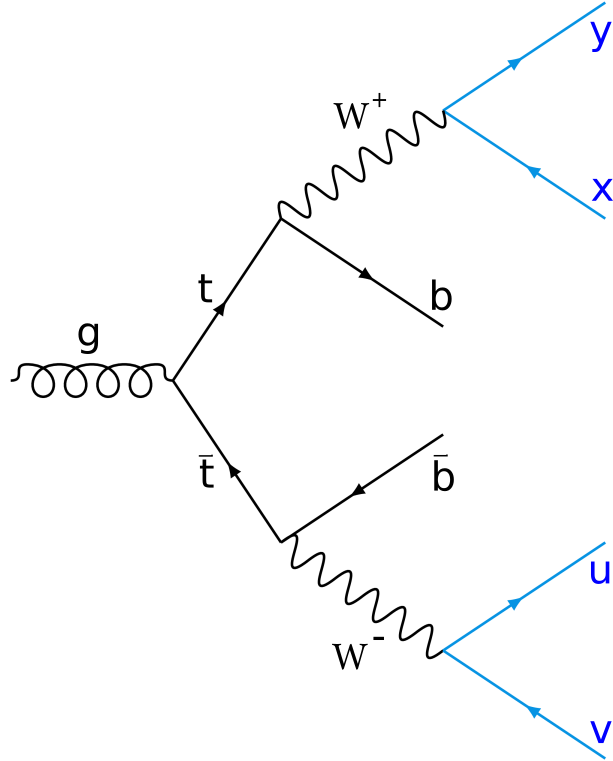
\includegraphics[width=0.3\linewidth]{Pics/cp1/Decay}
	\caption{Schematic decay of a $t\bar{t}$ pair. In the final decay state, the pairs xy and uv can be either quark or lepton pairs.  }
	\label{fig:Decay}
\end{figure}

 Based on the decays of the $W$-boson, the top-quark decay can be classified into three different decay channels, which are used for separate analyses, taking the specific signature inside the detector and the different background contaminations into account. The different decay channels are introduced below and  the corresponding branching ratios are given in~\cref{tab:T22}. The total decay chain is illustrated in~\cref{fig:Decay}, where the  $t\bar{t}$ pair is produced via  gluon-gluon fusion and  decays into the objects, which can finally be observed with the experimental equipment. The nature of these objects characterise the decay channel. They are denoted by the pairs x,y and u,v, which can either by a lepton or a quark pair.




\subsubsection{The all-hadronic decay channel}
In the fully hadronic decay channel (all-jets), both $W$-bosons from the $t\bar{t}$ final state decay hadronically into quarks. This is the dominant decay process for $t\bar{t}$ events. 

 Inside the detector, the signal of this decay is characterized by six jets. There are two jets  from the bottom quarks ($b$-jets), plus four lighter jets from the hadronic $W$-boson decays. The dominant background  for this decay channel stems from QCD-multijet events.

\subsubsection{The dileptonic decay channel}
With a branching ratio of just 10.5\% the dileptonic decay (dilepton) of both $W$-bosons is the smallest decay channel. 

 In the detector, this channel can be identified by a  signature with two $b$-jets from the top decays, two isolated charged leptons of opposite charge and a large amount of missing transverse energy, which is  a consequence of the two neutrinos.
The missing energy makes the reconstruction of this event topology particularly difficult. While QCD-multijet events do not play an important role, the dileptonic decay channel suffers from background from $Z$-boson events with extra jets in the final state.   

\subsubsection{The lepton + jets  decay channel}
The channel which is subject of the studies presented here, is  known as lepton + jets decay channel. One $W$-boson decays hadronically and  the other one leptonically, which offers significant advantages for the event selection and reconstruction. The leptonic  part of the decay helps to improve the identification of the interesting   events, while for the full kinematic reconstruction of the event the hadronic contributions are used in addition to the leptonic decay. 

 The detector signature consists of two $b$-jets and two lighter jets, one isolated charged lepton and a certain amount of missing transverse energy from the neutrino. Final states with a $W$-boson plus jets are the main background contribution for this decay channel.   
  

 \begin{center}
\captionof{table}{  Integrated branching ratios of the different top-quark pair decay channels~\cite{Olive:2016xmw}. }\label{tab:T22}

	
\vspace{0.3cm}	
	

\begin{tabular}{>{\centering}m{3.5cm}>{\centering}m{7.5cm} >{\centering}m{3.5cm} } \toprule

Decay channel& & Branching ratio&
\midrule
all-hadronic&$pp\rightarrow t\bar{t}\rightarrow W^+bW^-\bar{b}\rightarrow bq\bar{q'} \bar{b}q\bar{q'}$	&45.7\% &
dilepton	&$ pp\rightarrow t\bar{t}\rightarrow W^+bW^-\bar{b}\rightarrow bl\bar{\nu} \bar{b}\bar{l}\nu$&10.5\% &
lepton + jets		& $pp\rightarrow t\bar{t}\rightarrow W^+bW^-\bar{b}\rightarrow bl\bar{\nu} \bar{b}q\bar{q'}$&43.8\% &
\bottomrule
\end{tabular}

\end{center}
 \vspace{0.5cm} 
  
  
  
  
  
  
  
  
  
